\documentclass{notes}

\title{Geometrical considerations for the SPI module}
\author{Mathias Hoppe and Oskar Vallhagen}


\begin{document}
    \maketitle

    \noindent
    In this document we consider the geometry used to track pellet shards in the
    SPI module of \DREAM, and how that geometry relates to the magnetic field
    geometry used elsewhere in \DREAM.

    The SPI module uses a cartesian coordinate system with origin on the
    magnetic axis. The coordinate system is oriented such that the $z$ direction
    is parallel to the toroidal direction in $x=y=0$, as illustrated in
    figure~\ref{fig:geom}.

    \begin{figure}
        \centering
        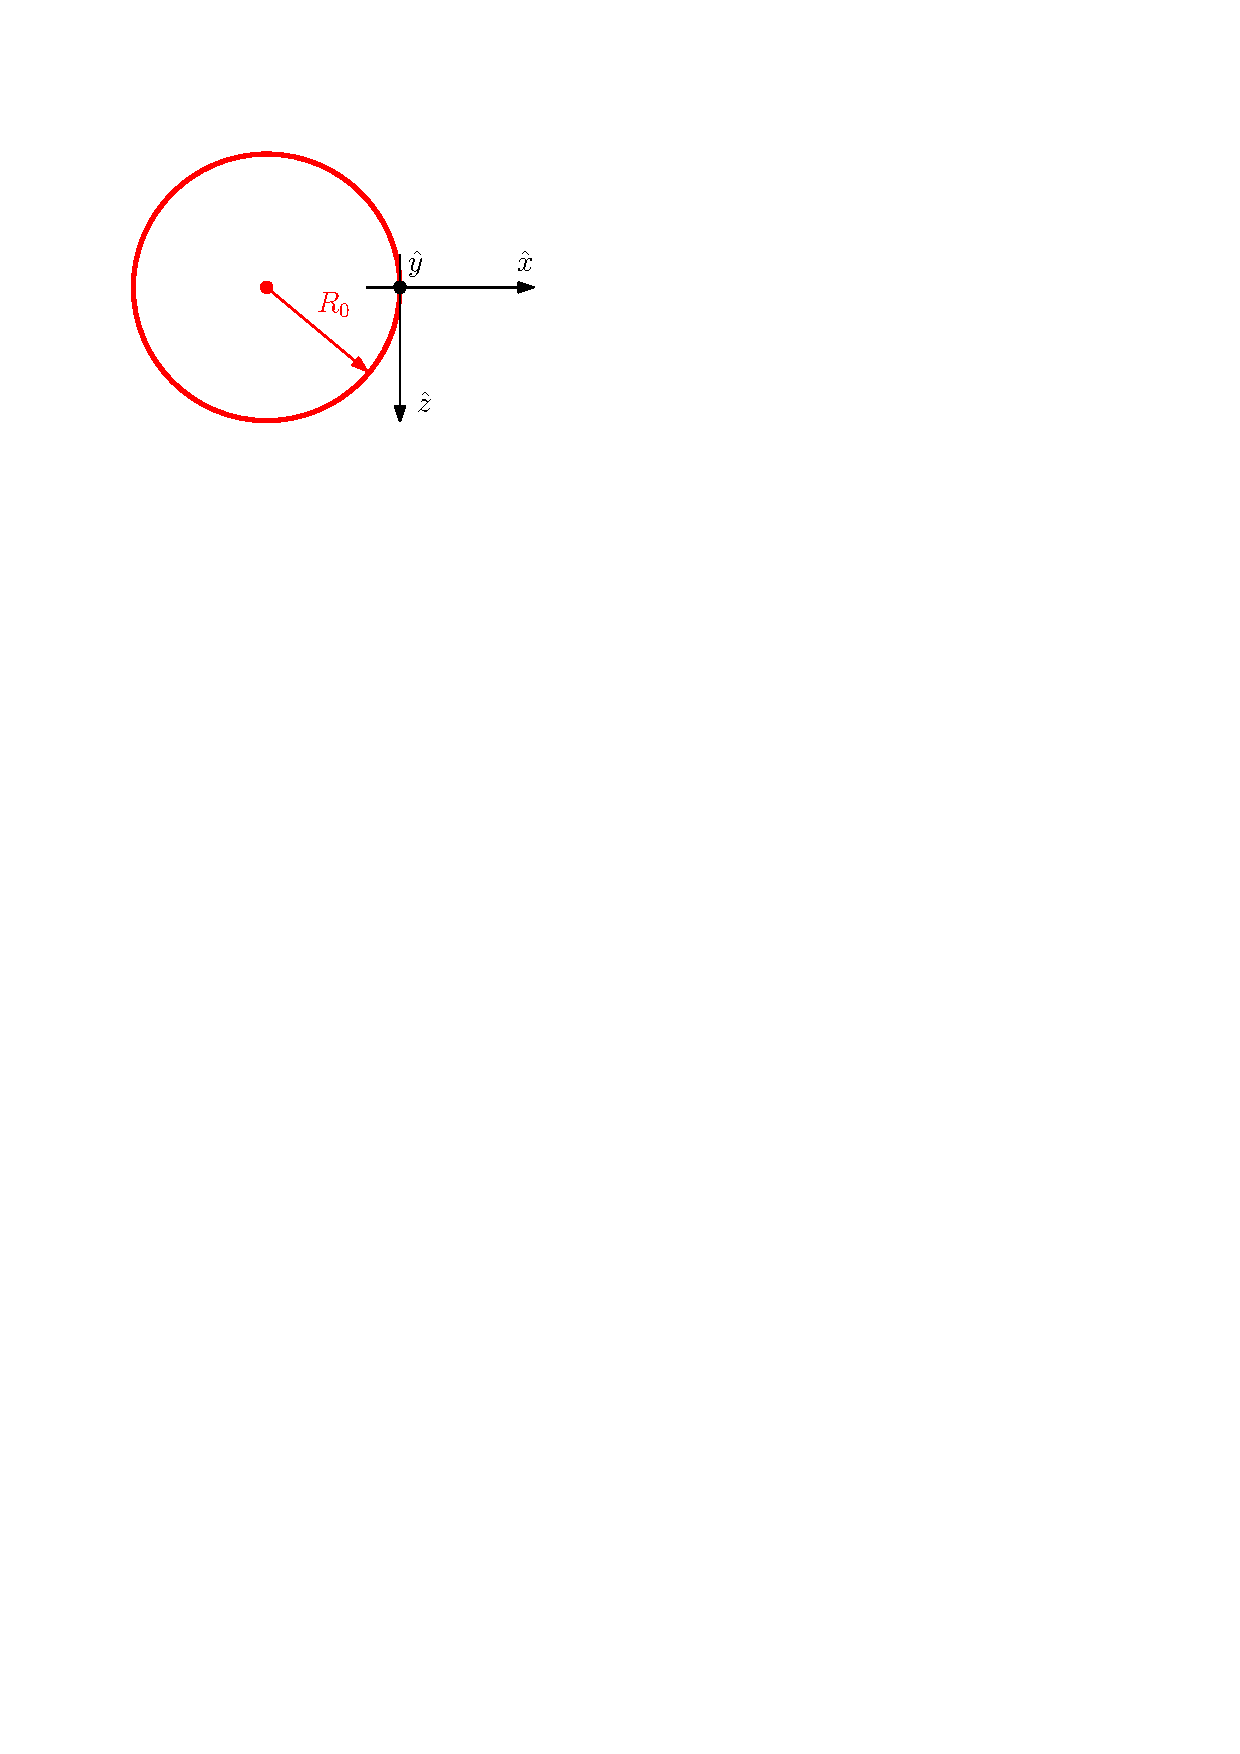
\includegraphics[width=0.5\textwidth]{figs/SPIgeom.pdf}
        \caption{
            Illustration of the coordinate system used for the SPI module in
            \DREAM.
        }
        \label{fig:geom}
    \end{figure}

    \section{Coordinate transformations}
    In the SPI module, it is necessary to map the cartesian coordinates
    $(x,y,z)$ of the points in space to the corresponding flux surface label
    $r$. In the toroidal case, this requires a two-step procedure where the
    cartesian coordinates $(x,y,z)$ are first transformed to their corresponding
    cylindrical $(R,Z,\varphi)$ or toroidal coordinates $(\rho,\theta,\varphi)$.
    In the second step, the cylindrical or toroidal coordinates must then be
    inverted to obtain the flux surface label $r$, and this generally requires
    numerical root-finding.

    \subsection{Cylindrical coordinates}
    The transformation to cylindrical coordinates is straightforward: since
    $x$ and $z$ lie in the horizontal plane, while $y$ is always vertical, the
    major radius and vertical position $Z$ is given by
    \begin{subequations}
        \begin{align}
        R &= \sqrt{(x+R_0)^2 + z^2},\\
        Z &= y.
        \end{align}
    \end{subequations}

    \subsection{Toroidal coordinates}
    To obtain the toroidal coordinates $\rho$ and $\theta$, we first introduce
    the position vector $\vec{r} = (x+R_0,y,z)$, defined to originate in $y=0$
    on the axis of symmetry of the tokamak (the red dot in
    figure~\ref{fig:geom}). We then introduce the unit vector
    \begin{equation}
        \hat{r} = \frac{\left(\vec{r}\cdot\hat{x}\right)\hat{x} + \left(\vec{r}\cdot\hat{z}\right)\hat{z}}
        {\sqrt{\left(\vec{r}\cdot\hat{x}\right)^2 + \left(\vec{r}\cdot\hat{z}\right)^2}} =
        %
        \frac{(x+R_0)\hat{x} + z\hat{z}}{\sqrt{(x+R_0)^2+z^2}},
    \end{equation}
    which is the normalized projection of the position vector $\vec{r}$ to the
    horizontal plane. With these vectors, we can then obtain the minor radius
    vector $\vec{\rho}$ as
    \begin{equation}
        \vec{\rho} = \vec{r}-R_0\hat{r} =
        \left(x+R_0-\frac{(x+R_0)R_0}{\sqrt{\left(x+R_0\right)^2 + z^2}}\right)\hat{x}
        + y\hat{y}
        + \left(z-\frac{zR_0}{\sqrt{\left(x+R_0\right)^2 + z^2}}\right)\hat{z},
    \end{equation}
    and the magnitude of this vector is
    \begin{equation}
        \rho = \sqrt{
            \left(x+R_0-\frac{(x+R_0)R_0}{\sqrt{\left(x+R_0\right)^2 + z^2}}\right)^2
            + y^2
            + \left(z-\frac{zR_0}{\sqrt{\left(x+R_0\right)^2 + z^2}}\right)^2
        }.
    \end{equation}
    Knowing the minor radius $\rho$ corresponding to $(x,y,z)$ will get us only
    part of the way to determining the flux surface radius $r$. To fully
    determine it, we also need to know the poloidal angle $\theta$ of the
    cartesian coordinates. In numerical geometry, this is easy to obtain from
    the minor radius vector $\vec{\rho}$. By the definition of the poloidal
    angle $\theta$ in numerical toroidal geometry, we have
    \begin{equation}
        \tan\theta = \frac{\left(\vec{\rho}\cdot\hat{y}\right)\mathrm{sgn}\left(R-R_0\right)}
            {\sqrt{\left(\vec{\rho}\cdot\hat{x}\right)^2 + \left(\vec{\rho}\cdot\hat{z}\right)^2}}
        %
        = \frac{y\,\mathrm{sgn}\left(R-R_0\right)}{\sqrt{
            \left(x+R_0-\frac{(x+R_0)R_0}{\sqrt{\left(x+R_0\right)^2 + z^2}}\right)^2
            + \left(z-\frac{zR_0}{\sqrt{\left(x+R_0\right)^2 + z^2}}\right)^2
        }},
    \end{equation}
    with
    \begin{equation}
        R = \sqrt{(x+R_0)^2+z^2}.
    \end{equation}
    The sign function appears since
    $\sqrt{(\vec{\rho}\cdot\hat{x})^2 + (\vec{\rho}\cdot\hat{z})^2}$
    should correspond to the horizontal cartesian coordinate in the poloidal
    plane (which is negative in the second and third quadrants).
    
    \section{Cylindrical coordinates to analytic B}
    The conversion from cartesian coordinates to flux surface coordinates in the analytical B-field geometry in DREAM is most easily done via a transformation to cylindrical coordinates. The reason for this is that the poloidal angle $\theta$ does not have a simple geometrical definition in this context.
    
    The flux surface geometry in the analytic B mode is related to the cylindrical coordinates according to
    \begin{align}
R &= R_0 + \Delta(r) + r\cos[\theta +\delta(r) \sin\theta], \nonumber \\
Z &= r \kappa(r) \sin\theta,
\label{eq:analyticB system}
\end{align}
where $\kappa$ is the elongation, $\Delta$ the Shafranov shift and $\delta$ a triangularity parameter. We solve this equation system by eliminating the $\theta$-dependence from the equation for $R$ using the equation for $Z$, and in that way obtain an equation for $r$ alone which is straightforward to solve numerically. First, we rewrite the equation for $R$ in terms of $\cos{\theta}$ and $\sin{\theta}$ rather than $\theta$ itself:
	\begin{equation}
		R = R_0 + \Delta (r) + r[\cos{\theta}\cos{(\delta(r)\sin{\theta})} - \sin{\theta}\sin{(\delta(r)\sin{\theta})}].
		\label{eq:RAnalyticB}
	\end{equation}
	From the equation for $Z$, we have
	\begin{align}
		\sin{\theta} &= \frac{Z}{r\kappa(r)}\nonumber \\
		\cos{\theta} &= \pm \sqrt{1-\left(\frac{Z}{r\kappa(r)}\right)^2}.
		\label{eq:SinCosAnalyticB}
	\end{align}
	It remains now to determine the sign on $\cos{\theta}$. We do this by calculating the major radius $R_\mathrm{crit}$ where $\cos{\theta}=0$. As the major radius is a monotonically increasing function of $\cos{\theta}$ {\color{red}(which holds as long as $\delta < 1$, but this might be necessary to not violate other assumptions, such as monotonically varying B-fields between the two extreme points on a flux surface?)}, if $R>R_\mathrm{crit}$, $\cos{\theta}>0$, and vice versa. The critical major radius is calculated by noting that when $\cos{\theta}=0$, we have $\sin{\theta}=1$, so that
	\begin{equation}
		R_\mathrm{crit} = R_0 + \Delta(r_\mathrm{min}) - r_\mathrm{min}\sin{(\delta(r_\mathrm{min}))},
	\end{equation}
	where $r_\mathrm{min}$ is calculated (numerically) from
	\begin{equation}
		Z = r_\mathrm{min}\kappa(r_\mathrm{min}).
	\end{equation}
	With the sign of $\cos{\theta}$ known, we can finally obtain an equation with $r$ as the only unknown by inserting equation \eqref{eq:SinCosAnalyticB} into equation \eqref{eq:RAnalyticB}. As the derivative of this equation with respect to $r$ diverges at $r=r_\mathrm{min}$, it is probably best to solve this equation using a bisection method rather than a Newton method.
	
\section{Minimum $r$ along a shard path}
To evaluate the time averaged delta function source, it is necessary to know the value of the smallest $r$ along the shard paths \footnote{More details about the delta function source can be found in appendix A of O. Vallhagen's master's thesis or in \texttt{doc/notes/SPIDeltaSource.pdf}}. The reason for this is that the flux surface label $\rho _\mathrm{p}$ \footnote{Not to be confused with the minor radius denoted $\rho$ without subscript. We use this notation here to be consistent with O. Vallhagen's master's thesis} of a shard varies non-monotonically during the time step where it passes its minimum value $\rho _\mathrm{p,closest}$ (which is technically only closest to the magnetic axis when the cross section has a circular shape). This means that the kernel can not simply be described by a box-like function bounded by the values of $r$ at the beginning and the end of the timestep. Instead, this timestep is divided in two parts, before and after the passing of $\rho _\mathrm{p,closest}$.

To see if $\rho _\mathrm{p,closest}$ has been passed during the current time step, we check whether the projection of the shard trajectory on the gradient of the radial coordinate has changed sign, i.e.~if
\begin{equation}
	[\mathbf{x}_\mathrm{p}(t)\cdot \nabla r(\mathbf{x}_\mathrm{p}(t))] \cdot [\mathbf{x}_\mathrm{p}(t+\Delta t)\cdot \nabla r(\mathbf{x}_\mathrm{p}(t+\Delta t))]<0,
\end{equation}
where $\mathbf{x}_\mathrm{p}(t)$ is the cartesian position vector of the shard. If this condition is satisfied, we proceed by finding $\rho _\mathrm{p,closest}$ by first parameterising the line between $\mathbf{x}_\mathrm{p}(t)$ and $\mathbf{x}_\mathrm{p}(t+\Delta t)$ with a parameter $\tau$ ($0<\tau<1$) as
\begin{equation}
	\bar{\mathbf{x}}_\mathrm{p}(\tau) = \mathbf{x}_\mathrm{p}(t) + \tau [\mathbf{x}_\mathrm{p}(t+\Delta t) - \mathbf{x}_\mathrm{p}(t)].
\end{equation} 
We can then find $\rho _\mathrm{p,closest}$ by solving
\begin{equation}
	\frac{\partial \rho _\mathrm{p}(\bar{\mathbf{x}}_\mathrm{p}(\tau))}{\partial \tau} = \nabla \rho _\mathrm{p} \cdot [\mathbf{x}_\mathrm{p}(t+\Delta t) - \mathbf{x}_\mathrm{p}(t)].
\end{equation}
Thus, if we can evaluate $\nabla \rho _\mathrm{p}$, we have an equation with $\tau$ as the only unknown, which is straight forward to solve with e.g. a bisection scheme. 

\subsection{$\nabla r$ with analytic B geometry}
The easiest way to evaluate $\nabla \rho _\mathrm{p}$ in analytic B geometry is to convert $\bar{\mathbf{x}}_\mathrm{p}(\tau)$ to flux surface coordinates (with the functionality implemented according to the above sections in this document), and then express $\nabla \rho _\mathrm{p}$ in terms of the flux surface coordinates. With analytic B geometry, according to \texttt{doc/notes/theory.pdf}, this can be done as (here with $r=\rho _\mathrm{p}$)
\begin{align}
\nabla r &= \frac{\frac{\partial z}{\partial \theta} (\cos{\varphi}\hat{x} + \sin{\varphi}\hat{y}) - \frac{\partial R}{\partial \theta} \hat{z}}{\frac{\partial R}{\partial r}\frac{\partial z}{\partial \theta} - \frac{\partial R}{\partial \theta}\frac{\partial z}{\partial r}},
\end{align}
where
\begin{align}
\frac{\partial R}{\partial r} &= \Delta' + \cos[\theta+\delta\sin\theta]-r\delta'\sin\theta\sin[\theta+\delta\sin\theta], \nonumber \\
\frac{\partial R}{\partial \theta} &= -r(1+\delta\cos\theta)\sin[\theta+\delta\sin\theta],  \nonumber \\
\frac{\partial z}{\partial r} &=  \kappa\left(1+ \frac{r\kappa'}{\kappa}\right)\sin\theta, \nonumber \\
\frac{\partial z}{\partial \theta} &= r\kappa\cos\theta.
\end{align}
	

    
\end{document}
